\section{Conclusion}
As seen in Section~\ref{sec:soa_benchmarking} of state of art, a successful benchmark faces three challenges: reproducibility, accuracy, and representativeness. 
This chapter has covered two of the three criteria.

The first section covered the reproducibility challenge by studying the existing reproducibility techniques. We have observed that there are two primary methods for encapsulating experimental systems, the first is to utilize virtual machines, and the second is based on containers. We established that Docker is more suitable for energy-related studies for three reasons.

\begin{enumerate}
    \item It is more lightweight than virtual machines.
    \item It offers interactivity with the hardware of the host machine, which will enable us to gather more metrics.
    \item It has a constant overhead, a key factor to nullify the encapsulation impact on the energy consumption when performing empirical analyses.
\end{enumerate}

After settling on the most suitable choice to encapsulate experiments, we highlighted the need to enhance the reproducibility of empirical tests along several axes (benchmarks, metrics, and candidates) to keep up with the rapid pace of software development. 
Furthermore, we have provided a model that enables comparative experiment \emph{extension}.
The foundation of this model is separating the experiment into multiple independent components: an orchestrator that executes the experiment, one or more observers that collect metrics, the candidates being tested, and the benchmark against which these candidates are being compared.

As for the second section, we addressed the accuracy challenge in energy-based experiments.
We started by analyzing the impact of the chosen encapsulation method from the previous section on this challenge to determine that the impact is negligible.
Then, we conducted an empirical study utilizing some of the well-known benchmarks in literature, \texttt{Stress-ng}~\footnote{\url{https://kernel.ubuntu.com/~cking/stress-ng}} and \texttt{NAS Parallel Benchmark}~\cite{Bailey:1991:NPB:125826.125925}, on a variety of machines with diverse hardware combinations and operating system setups and tunings. We have shown that optimizing the operating system can significantly affect how accurately energy is used. This effect can affect the accuracy of the experiments from an increase of $5\times$ to a penalty of $30\times$.

We have also shown in this section the harm that this taming of the variation can cause to the representativeness of the results since some aspects that help increase the accuracy of the results in the research environment cannot be applied in the production environment, such as turning off the C-states. Another impact of increasing this accuracy was the increase in the overall energy consumption of the tests. Even if the overall was for all the candidates, this remains an issue to be addressed.

This chapter aims to establish a reproducible and accurate protocol for conducting energy-related experiments. From now on, we shall use this protocol in our studies to reduce software energy usage.





%  THIS SHOULD BE WITHIN THE perspective chapter 
% By the end of this study, we have gathered enough guidelines to make the tests more reproducible, accurate and extensible.
% We created a set of new tests named \textbf{energy tests} which are more similar to performance tests.
% Thanks to the work of two interns [Mamadou and Adrien] we created a CI/CD platform to measure the energy consumption of Java projects and we could track the evolution of the this energy across different stages of the project.
% In the figure below we see an example of this plugin.
% For more details please visit the gitlab repository\footnote{\url{https://gitlab.inria.fr/mamdiall/J-Joules}}~\footnote{\url{https://gitlab.inria.fr/mamdiall/jjoules-plugin}} .


% \begin{figure}%[!htb]
%     \center{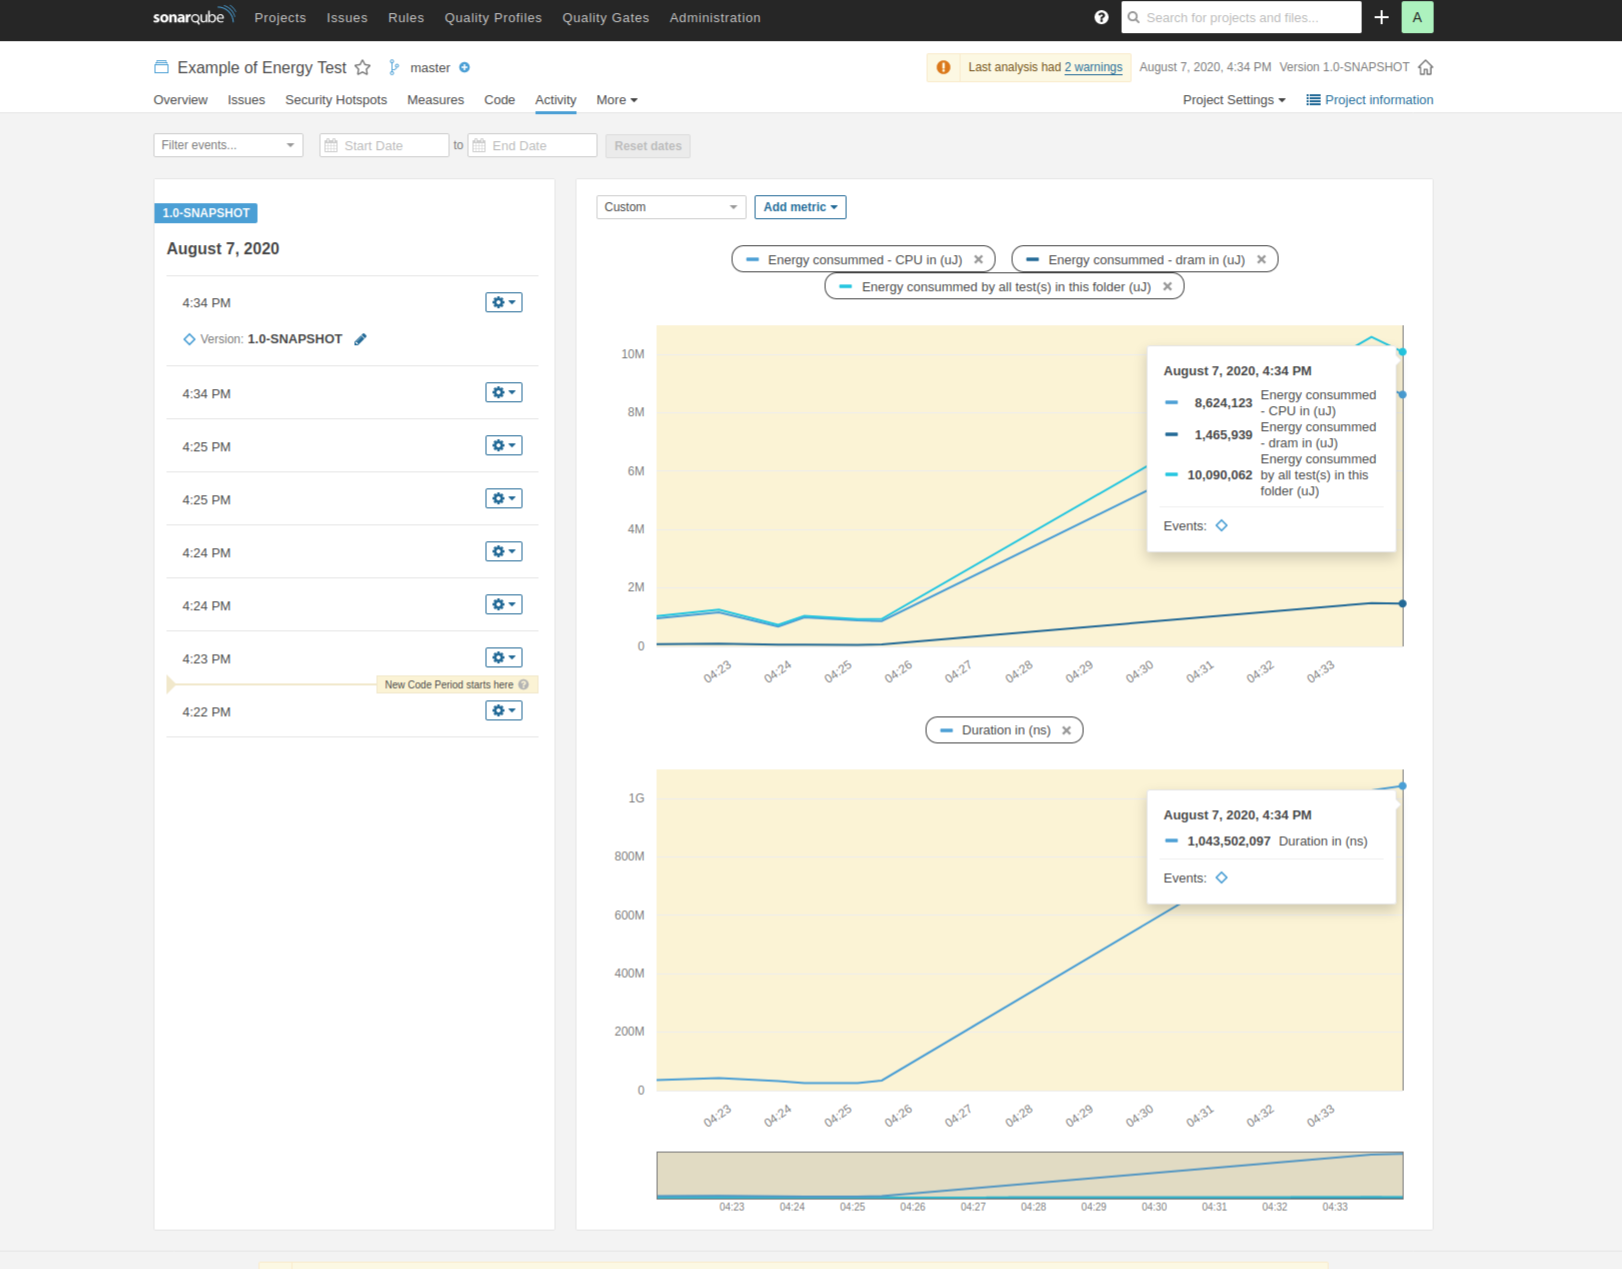
\includegraphics[width=.9\linewidth]{imgs/JunitSonarplugin}}
%     \caption{Example of the Junit Sonar Plugin}\label{fig:sonar_plugin}
% \end{figure}
